% Created 2020-04-23 Thu 16:45
% Intended LaTeX compiler: pdflatex
\documentclass[bigger]{beamer}
\usepackage[utf8]{inputenc}
\usepackage[T1]{fontenc}
\usepackage{graphicx}
\usepackage{grffile}
\usepackage{longtable}
\usepackage{wrapfig}
\usepackage{rotating}
\usepackage[normalem]{ulem}
\usepackage{amsmath}
\usepackage{textcomp}
\usepackage{amssymb}
\usepackage{capt-of}
\usepackage{hyperref}
\usepackage{natbib}
\usepackage{bm}
\usepackage{pgfplots}
\usepgfplotslibrary{groupplots,dateplot}
\usetikzlibrary{patterns,shapes.arrows}
\pgfplotsset{compat=newest}
\usepackage{dsfont}
\usepackage{xcolor}
\usepackage{listings}
\DeclareMathOperator{\TopHat}{TH}
\DeclareMathOperator{\CDF}{CDF}
\usetheme{Madrid}
\author{Aleksandr Petrosyan}
\date{\today}
\title{Cosmological Parameter estimation using Bayesian accelerated Machine learning.}
\hypersetup{
 pdfauthor={Aleksandr Petrosyan},
 pdftitle={Cosmological Parameter estimation using Bayesian accelerated Machine learning.},
 pdfkeywords={},
 pdfsubject={},
 pdfcreator={Emacs 26.3 (Org mode 9.1.9)}, 
 pdflang={English}}
\begin{document}

\maketitle

\begin{frame}[label={sec:orge6b6c72}]{What is \(\Lambda\)CDM.}
It's the accepted standard model of Cosmology. 
Has the following main parameters:
\begin{itemize}
\item \(\Omega_{b}h^{2}\) --- Physical baryon density.
\item \(\Omega_{c}h^{2}\) --- Physical dark matter density.
\item \(\tau_{0}\) --- Age of the universe.
\item \(n_{s}\) --- Scalar spectral index.
\item \(\tau_\text{reio}\) --- Re-ionization optical depth.
\item \(\Delta_{R}^{2}\) --- Curvature fluctuation amplitude.
\end{itemize}
\end{frame}

\begin{frame}[label={sec:orga7c365a}]{How do we measure it?}
Have Planck, WMap and many other sources of data.

Do Bayesian inference. Long discussion what this actually means. 

The gist: 
\begin{itemize}
\item Data using \(\chi^{2}\)defines \({\cal L}\) --- likelihood.
\item Prior information (other experiments) give us \(\pi\) --- the prior.
\item From Bayes' theorem, compute \emph{evidence} \({\cal Z}\) and \emph{posterior} \({\cal P}\).
\item From posterior, \emph{marginalise} the \emph{calibration parameters}.
\end{itemize}
\end{frame}

\begin{frame}[label={sec:orgf5b3dfe}]{Example of posterior.}
  Started with a \alert{Gaussian}. Then Gave an \alert{offset}.
  \(\ln {\cal Z} = -62 \pm 1\) exactly what we expect. Except for
  \alert{one} case.
  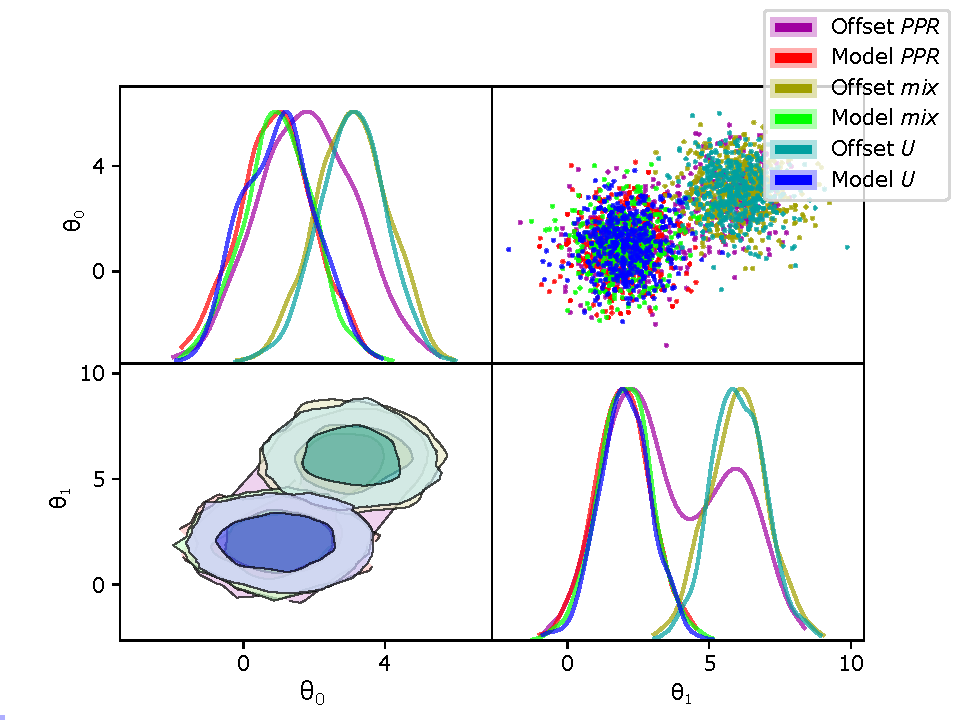
\includegraphics[width=.75\linewidth]{./illustrations/convergence.pdf}
  
\end{frame}
\begin{frame}[label={sec:org083fab8}]{How do we do it?}
We are spoiled for choice. But can only use Monte-Carlo in many
dimensions (lots of parameters).

The fastest methods given below in order of stability/speed. 
\begin{block}{Monte-Carlo methods}
\begin{itemize}
\item Nested sampling.
\item Hamiltonian Monte-Carlo.
\item Metropolis-Hastings.
\end{itemize}
\end{block}
\end{frame}


\begin{frame}[label={sec:orgcf084f1}]{Can we make it go fast?}
Yes and no. 

If we give the prior as the posterior, we will converge the
fastest. But the evidence is all wrong. The posterior is also wrong. 

We can mitigate this, by using an \emph{intuitive Gaussian}. But it gets
the wrong answer if we were wrong about either the place or the size
of the Posterior.
\begin{block}{My Intuitive Gaussian.}
Take \(\tilde{\pi}(\theta) = {\cal P}(\theta)\), change \({\cal L}\), such that. 
\begin{equation*}
\tilde{\cal L}(\theta)\tilde{\pi}(\theta) = {\cal L}(\theta)\pi(\theta)
\end{equation*}
\end{block}
\end{frame}



\begin{frame}[label={sec:org958d1e9}]{Can we safely make it go fast? Posterior re-partitioning.}

\begin{block}{Chen-Ferroz-Hobson PPR.}
\begin{equation*}
\tilde{\pi}(\bm{\bm{\theta}};\beta) = \cfrac{\pi(\bm{\theta})^{\beta}}{Z(\beta)\{\pi\}},
\end{equation*}
\begin{equation*}
 Z(\beta)\{\pi\} = \int_{\bm{\theta} \in \Psi}		\pi(\bm{\bm{\theta}})^{\beta}d\bm{\bm{\theta}}.
 \end{equation*}
\begin{equation*}
\tilde{\cal L}(\bm{\theta}) = {\cal L}(\bm{\theta}) Z(\beta)\{\pi\} \cdot		\pi^{1-\beta}(\bm{\theta}).
\end{equation*}
\end{block}
This can mitigate the issues of size, but not place.

\end{frame}



\begin{frame}[label={sec:org73e18f6}]{Works well, but not if we have an offset.}
\begin{center}
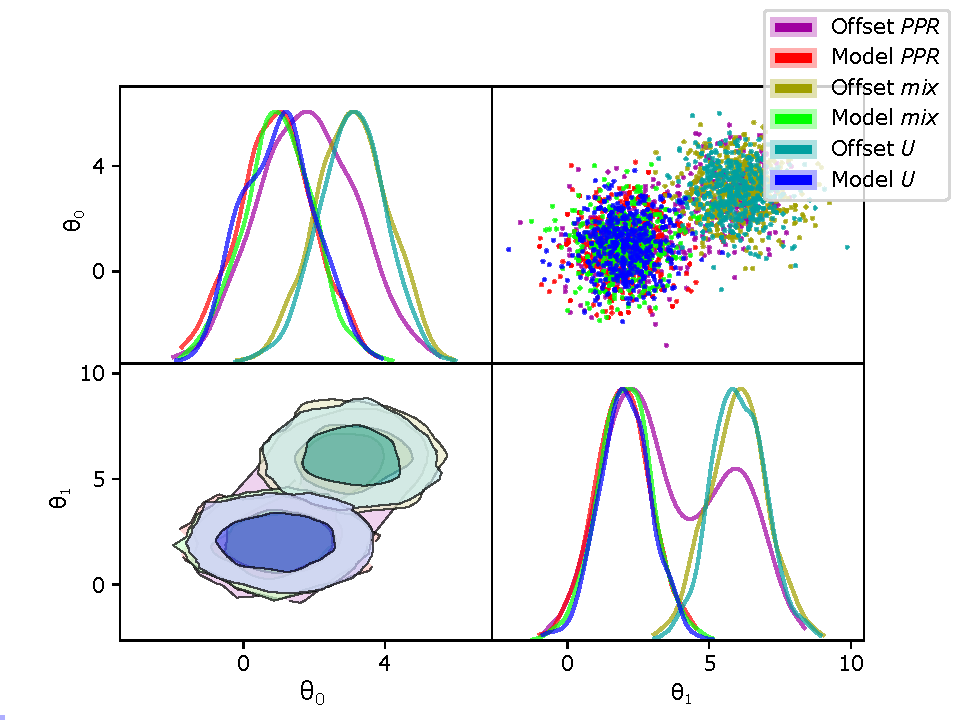
\includegraphics[width=.9\linewidth]{./illustrations/convergence.pdf}
\end{center}
\end{frame}

\begin{frame}[label={sec:orgb21b8c0}]{My discovery.}
\begin{block}{My Stochastic superpositional isometric model mixture.}
\begin{equation*}
  \tilde{\pi}(\bm{\theta}; \beta)  \triangleq \begin{cases}
	\tilde{\pi}_{1}(\bm{\theta}) & \text{with probability } \beta_{1},\\
	& \vdots,\\
	\tilde{\pi}_{n}(\bm{\theta}) & \text{with probability } (1- \sum_{i}^{m}\beta_{i}),
	\end{cases}
\end{equation*}
\begin{equation*}
  \tilde{\cal L}(\bm{\theta}; \bm{\beta})  \triangleq
  \begin{cases}
	\tilde{\cal L}_{1}(\bm{\theta}) &  \text{with probability } \beta_{1},\\
		    &\vdots,\\
	\tilde{\cal L}_{m}(\bm{\theta}) & \text{with probability} (1- \sum_{i}^{m}\beta_{i}).
\end{cases}
\end{equation*}
\begin{equation*}
  \tilde{\pi}(\bm{\theta}; \bm{\beta}) = \tilde{\pi}(\bm{\theta})_{i} \Leftrightarrow \tilde{\cal L}(\bm{\theta}; \bm{\beta}) = \tilde{\cal L}_{m}(\bm{\theta}; \bm{\beta}), 
\end{equation*}
\end{block}
\end{frame}

\begin{frame}
  \frametitle{This is what it looks like}
  % This file was created by tikzplotlib v0.9.1.
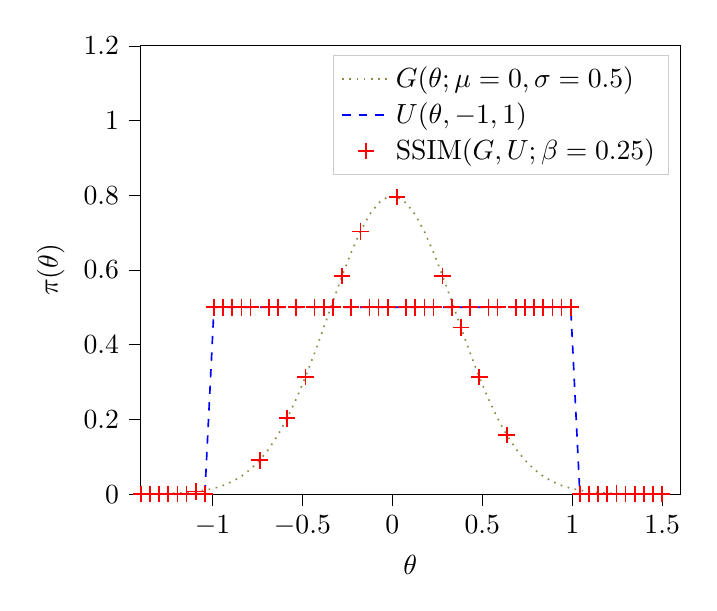
\begin{tikzpicture}

\begin{axis}[
legend cell align={left},
legend style={fill opacity=0.8, draw opacity=1, text opacity=1, draw=white!80!black},
tick align=outside,
tick pos=left,
x grid style={white!69.0196078431373!black},
xlabel={\(\displaystyle \theta\)},
xmin=-1.4, xmax=1.6,
xtick style={color=black},
y grid style={white!69.0196078431373!black},
ylabel={\(\displaystyle \pi(\theta)\)},
ymin=0, ymax=1.2,
ytick style={color=black}
]
\addplot [semithick, yellow!50!black, dotted]
table {%
-1.5 9.8466777332468e-05
-1.44915254237288 0.0001793872435764
-1.39830508474576 0.000320118348094559
-1.34745762711864 0.000559560121531124
-1.29661016949153 0.000958076356441112
-1.24576271186441 0.00160683272401611
-1.19491525423729 0.00263972321036136
-1.14406779661017 0.00424779248787262
-1.09322033898305 0.00669553635076534
-1.04237288135593 0.0103377167883577
-0.991525423728814 0.015634394496712
-0.940677966101695 0.0231608599466659
-0.889830508474576 0.0336082170150122
-0.838983050847458 0.0477698022564135
-0.788135593220339 0.066508720415643
-0.73728813559322 0.0907028470877726
-0.686440677966102 0.121165903387615
-0.635593220338983 0.15854666388776
-0.584745762711864 0.203212757823817
-0.533898305084746 0.255130282294824
-0.483050847457627 0.313754690902936
-0.432203389830508 0.377951108859794
-0.38135593220339 0.445962353038858
-0.330508474576271 0.515439801267037
-0.279661016949152 0.583545711433813
-0.228813559322034 0.647126211028834
-0.177966101694915 0.702943270974129
-0.127118644067796 0.747943415704262
-0.0762711864406778 0.77953278826435
-0.0254237288135593 0.795824323519198
0.0254237288135595 0.795824323519198
0.076271186440678 0.77953278826435
0.127118644067797 0.747943415704262
0.177966101694915 0.702943270974129
0.228813559322034 0.647126211028834
0.279661016949153 0.583545711433812
0.330508474576271 0.515439801267037
0.38135593220339 0.445962353038858
0.432203389830509 0.377951108859794
0.483050847457627 0.313754690902936
0.533898305084746 0.255130282294824
0.584745762711865 0.203212757823817
0.635593220338983 0.15854666388776
0.686440677966102 0.121165903387615
0.737288135593221 0.0907028470877724
0.788135593220339 0.0665087204156429
0.838983050847458 0.0477698022564135
0.889830508474577 0.0336082170150121
0.940677966101695 0.0231608599466659
0.991525423728814 0.015634394496712
1.04237288135593 0.0103377167883577
1.09322033898305 0.00669553635076532
1.14406779661017 0.00424779248787262
1.19491525423729 0.00263972321036135
1.24576271186441 0.0016068327240161
1.29661016949153 0.000958076356441112
1.34745762711864 0.000559560121531121
1.39830508474576 0.000320118348094558
1.44915254237288 0.000179387243576399
1.5 9.8466777332468e-05
};
\addlegendentry{$G(\theta; \mu=0, \sigma=0.5)$}
\addplot [semithick, blue, dashed]
table {%
-1.5 0
-1.44915254237288 0
-1.39830508474576 0
-1.34745762711864 0
-1.29661016949153 0
-1.24576271186441 0
-1.19491525423729 0
-1.14406779661017 0
-1.09322033898305 0
-1.04237288135593 0
-0.991525423728814 0.5
-0.940677966101695 0.5
-0.889830508474576 0.5
-0.838983050847458 0.5
-0.788135593220339 0.5
-0.73728813559322 0.5
-0.686440677966102 0.5
-0.635593220338983 0.5
-0.584745762711864 0.5
-0.533898305084746 0.5
-0.483050847457627 0.5
-0.432203389830508 0.5
-0.38135593220339 0.5
-0.330508474576271 0.5
-0.279661016949152 0.5
-0.228813559322034 0.5
-0.177966101694915 0.5
-0.127118644067796 0.5
-0.0762711864406778 0.5
-0.0254237288135593 0.5
0.0254237288135595 0.5
0.076271186440678 0.5
0.127118644067797 0.5
0.177966101694915 0.5
0.228813559322034 0.5
0.279661016949153 0.5
0.330508474576271 0.5
0.38135593220339 0.5
0.432203389830509 0.5
0.483050847457627 0.5
0.533898305084746 0.5
0.584745762711865 0.5
0.635593220338983 0.5
0.686440677966102 0.5
0.737288135593221 0.5
0.788135593220339 0.5
0.838983050847458 0.5
0.889830508474577 0.5
0.940677966101695 0.5
0.991525423728814 0.5
1.04237288135593 0
1.09322033898305 0
1.14406779661017 0
1.19491525423729 0
1.24576271186441 0
1.29661016949153 0
1.34745762711864 0
1.39830508474576 0
1.44915254237288 0
1.5 0
};
\addlegendentry{$U(\theta, -1, 1)$}
\addplot [semithick, red, mark=+, mark size=3, mark options={solid}, only marks]
table {%
-1.5 0
-1.44915254237288 0
-1.39830508474576 0
-1.34745762711864 0
-1.29661016949153 0
-1.24576271186441 0
-1.19491525423729 0
-1.14406779661017 0
-1.09322033898305 0.00669553635076534
-1.04237288135593 0
-0.991525423728814 0.5
-0.940677966101695 0.5
-0.889830508474576 0.5
-0.838983050847458 0.5
-0.788135593220339 0.5
-0.73728813559322 0.0907028470877726
-0.686440677966102 0.5
-0.635593220338983 0.5
-0.584745762711864 0.203212757823817
-0.533898305084746 0.5
-0.483050847457627 0.313754690902936
-0.432203389830508 0.5
-0.38135593220339 0.5
-0.330508474576271 0.5
-0.279661016949152 0.583545711433813
-0.228813559322034 0.5
-0.177966101694915 0.702943270974129
-0.127118644067796 0.5
-0.0762711864406778 0.5
-0.0254237288135593 0.5
0.0254237288135595 0.795824323519198
0.076271186440678 0.5
0.127118644067797 0.5
0.177966101694915 0.5
0.228813559322034 0.5
0.279661016949153 0.583545711433812
0.330508474576271 0.5
0.38135593220339 0.445962353038858
0.432203389830509 0.5
0.483050847457627 0.313754690902936
0.533898305084746 0.5
0.584745762711865 0.5
0.635593220338983 0.15854666388776
0.686440677966102 0.5
0.737288135593221 0.5
0.788135593220339 0.5
0.838983050847458 0.5
0.889830508474577 0.5
0.940677966101695 0.5
0.991525423728814 0.5
1.04237288135593 0
1.09322033898305 0
1.14406779661017 0
1.19491525423729 0
1.24576271186441 0.0016068327240161
1.29661016949153 0
1.34745762711864 0
1.39830508474576 0
1.44915254237288 0
1.5 0
};
\addlegendentry{SSIM$(G, U; \beta=0.25)$}
\end{axis}

\end{tikzpicture}

\end{frame}

\begin{frame}
  \frametitle{This is what it looks like}
% This file was created by tikzplotlib v0.9.1.
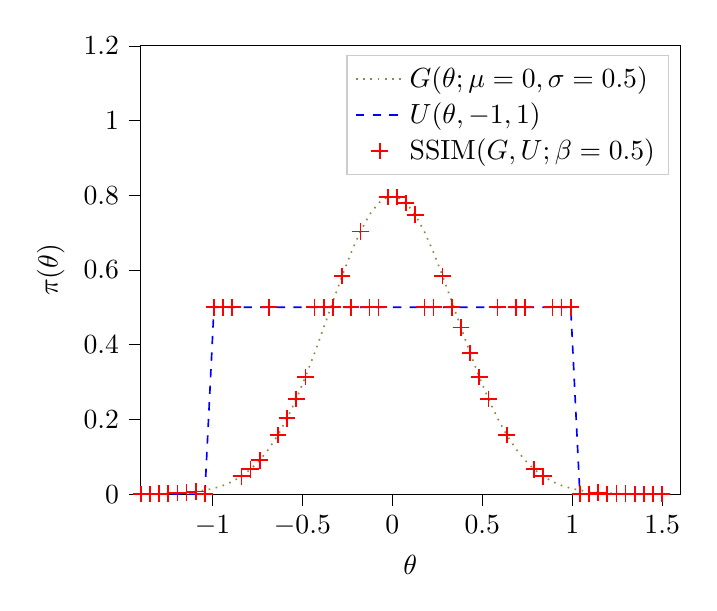
\begin{tikzpicture}

\begin{axis}[
legend cell align={left},
legend style={fill opacity=0.8, draw opacity=1, text opacity=1, draw=white!80!black},
tick align=outside,
tick pos=left,
x grid style={white!69.0196078431373!black},
xlabel={\(\displaystyle \theta\)},
xmin=-1.4, xmax=1.6,
xtick style={color=black},
y grid style={white!69.0196078431373!black},
ylabel={\(\displaystyle \pi(\theta)\)},
ymin=0, ymax=1.2,
ytick style={color=black}
]
\addplot [semithick, yellow!50!black, dotted]
table {%
-1.5 9.8466777332468e-05
-1.44915254237288 0.0001793872435764
-1.39830508474576 0.000320118348094559
-1.34745762711864 0.000559560121531124
-1.29661016949153 0.000958076356441112
-1.24576271186441 0.00160683272401611
-1.19491525423729 0.00263972321036136
-1.14406779661017 0.00424779248787262
-1.09322033898305 0.00669553635076534
-1.04237288135593 0.0103377167883577
-0.991525423728814 0.015634394496712
-0.940677966101695 0.0231608599466659
-0.889830508474576 0.0336082170150122
-0.838983050847458 0.0477698022564135
-0.788135593220339 0.066508720415643
-0.73728813559322 0.0907028470877726
-0.686440677966102 0.121165903387615
-0.635593220338983 0.15854666388776
-0.584745762711864 0.203212757823817
-0.533898305084746 0.255130282294824
-0.483050847457627 0.313754690902936
-0.432203389830508 0.377951108859794
-0.38135593220339 0.445962353038858
-0.330508474576271 0.515439801267037
-0.279661016949152 0.583545711433813
-0.228813559322034 0.647126211028834
-0.177966101694915 0.702943270974129
-0.127118644067796 0.747943415704262
-0.0762711864406778 0.77953278826435
-0.0254237288135593 0.795824323519198
0.0254237288135595 0.795824323519198
0.076271186440678 0.77953278826435
0.127118644067797 0.747943415704262
0.177966101694915 0.702943270974129
0.228813559322034 0.647126211028834
0.279661016949153 0.583545711433812
0.330508474576271 0.515439801267037
0.38135593220339 0.445962353038858
0.432203389830509 0.377951108859794
0.483050847457627 0.313754690902936
0.533898305084746 0.255130282294824
0.584745762711865 0.203212757823817
0.635593220338983 0.15854666388776
0.686440677966102 0.121165903387615
0.737288135593221 0.0907028470877724
0.788135593220339 0.0665087204156429
0.838983050847458 0.0477698022564135
0.889830508474577 0.0336082170150121
0.940677966101695 0.0231608599466659
0.991525423728814 0.015634394496712
1.04237288135593 0.0103377167883577
1.09322033898305 0.00669553635076532
1.14406779661017 0.00424779248787262
1.19491525423729 0.00263972321036135
1.24576271186441 0.0016068327240161
1.29661016949153 0.000958076356441112
1.34745762711864 0.000559560121531121
1.39830508474576 0.000320118348094558
1.44915254237288 0.000179387243576399
1.5 9.8466777332468e-05
};
\addlegendentry{$G(\theta; \mu=0, \sigma=0.5)$}
\addplot [semithick, blue, dashed]
table {%
-1.5 0
-1.44915254237288 0
-1.39830508474576 0
-1.34745762711864 0
-1.29661016949153 0
-1.24576271186441 0
-1.19491525423729 0
-1.14406779661017 0
-1.09322033898305 0
-1.04237288135593 0
-0.991525423728814 0.5
-0.940677966101695 0.5
-0.889830508474576 0.5
-0.838983050847458 0.5
-0.788135593220339 0.5
-0.73728813559322 0.5
-0.686440677966102 0.5
-0.635593220338983 0.5
-0.584745762711864 0.5
-0.533898305084746 0.5
-0.483050847457627 0.5
-0.432203389830508 0.5
-0.38135593220339 0.5
-0.330508474576271 0.5
-0.279661016949152 0.5
-0.228813559322034 0.5
-0.177966101694915 0.5
-0.127118644067796 0.5
-0.0762711864406778 0.5
-0.0254237288135593 0.5
0.0254237288135595 0.5
0.076271186440678 0.5
0.127118644067797 0.5
0.177966101694915 0.5
0.228813559322034 0.5
0.279661016949153 0.5
0.330508474576271 0.5
0.38135593220339 0.5
0.432203389830509 0.5
0.483050847457627 0.5
0.533898305084746 0.5
0.584745762711865 0.5
0.635593220338983 0.5
0.686440677966102 0.5
0.737288135593221 0.5
0.788135593220339 0.5
0.838983050847458 0.5
0.889830508474577 0.5
0.940677966101695 0.5
0.991525423728814 0.5
1.04237288135593 0
1.09322033898305 0
1.14406779661017 0
1.19491525423729 0
1.24576271186441 0
1.29661016949153 0
1.34745762711864 0
1.39830508474576 0
1.44915254237288 0
1.5 0
};
\addlegendentry{$U(\theta, -1, 1)$}
\addplot [semithick, red, mark=+, mark size=3, mark options={solid}, only marks]
table {%
-1.5 9.8466777332468e-05
-1.44915254237288 0.0001793872435764
-1.39830508474576 0
-1.34745762711864 0.000559560121531124
-1.29661016949153 0.000958076356441112
-1.24576271186441 0.00160683272401611
-1.19491525423729 0.00263972321036136
-1.14406779661017 0.00424779248787262
-1.09322033898305 0.00669553635076534
-1.04237288135593 0
-0.991525423728814 0.5
-0.940677966101695 0.5
-0.889830508474576 0.5
-0.838983050847458 0.0477698022564135
-0.788135593220339 0.066508720415643
-0.73728813559322 0.0907028470877726
-0.686440677966102 0.5
-0.635593220338983 0.15854666388776
-0.584745762711864 0.203212757823817
-0.533898305084746 0.255130282294824
-0.483050847457627 0.313754690902936
-0.432203389830508 0.5
-0.38135593220339 0.5
-0.330508474576271 0.5
-0.279661016949152 0.583545711433813
-0.228813559322034 0.5
-0.177966101694915 0.702943270974129
-0.127118644067796 0.5
-0.0762711864406778 0.5
-0.0254237288135593 0.795824323519198
0.0254237288135595 0.795824323519198
0.076271186440678 0.77953278826435
0.127118644067797 0.747943415704262
0.177966101694915 0.5
0.228813559322034 0.5
0.279661016949153 0.583545711433812
0.330508474576271 0.5
0.38135593220339 0.445962353038858
0.432203389830509 0.377951108859794
0.483050847457627 0.313754690902936
0.533898305084746 0.255130282294824
0.584745762711865 0.5
0.635593220338983 0.15854666388776
0.686440677966102 0.5
0.737288135593221 0.5
0.788135593220339 0.0665087204156429
0.838983050847458 0.0477698022564135
0.889830508474577 0.5
0.940677966101695 0.5
0.991525423728814 0.5
1.04237288135593 0
1.09322033898305 0
1.14406779661017 0.00424779248787262
1.19491525423729 0
1.24576271186441 0.0016068327240161
1.29661016949153 0.000958076356441112
1.34745762711864 0
1.39830508474576 0.000320118348094558
1.44915254237288 0
1.5 9.8466777332468e-05
};
\addlegendentry{SSIM$(G, U; \beta=0.5)$}
\end{axis}

\end{tikzpicture}

\end{frame}


\begin{frame}
  \frametitle{This is what it looks like}
  % This file was created by tikzplotlib v0.9.1.
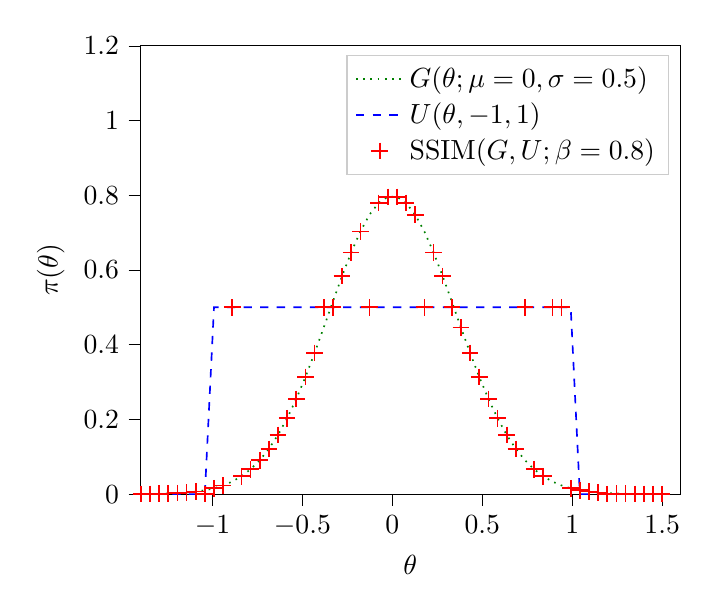
\begin{tikzpicture}

\begin{axis}[
legend cell align={left},
legend style={fill opacity=0.8, draw opacity=1, text opacity=1, draw=white!80!black},
tick align=outside,
tick pos=left,
x grid style={white!69.0196078431373!black},
xlabel={\(\displaystyle \theta\)},
xmin=-1.4, xmax=1.6,
xtick style={color=black},
y grid style={white!69.0196078431373!black},
ylabel={\(\displaystyle \pi(\theta)\)},
ymin=0, ymax=1.2,
ytick style={color=black}
]
\addplot [semithick, green!50!black, dotted]
table {%
-1.5 9.8466777332468e-05
-1.44915254237288 0.0001793872435764
-1.39830508474576 0.000320118348094559
-1.34745762711864 0.000559560121531124
-1.29661016949153 0.000958076356441112
-1.24576271186441 0.00160683272401611
-1.19491525423729 0.00263972321036136
-1.14406779661017 0.00424779248787262
-1.09322033898305 0.00669553635076534
-1.04237288135593 0.0103377167883577
-0.991525423728814 0.015634394496712
-0.940677966101695 0.0231608599466659
-0.889830508474576 0.0336082170150122
-0.838983050847458 0.0477698022564135
-0.788135593220339 0.066508720415643
-0.73728813559322 0.0907028470877726
-0.686440677966102 0.121165903387615
-0.635593220338983 0.15854666388776
-0.584745762711864 0.203212757823817
-0.533898305084746 0.255130282294824
-0.483050847457627 0.313754690902936
-0.432203389830508 0.377951108859794
-0.38135593220339 0.445962353038858
-0.330508474576271 0.515439801267037
-0.279661016949152 0.583545711433813
-0.228813559322034 0.647126211028834
-0.177966101694915 0.702943270974129
-0.127118644067796 0.747943415704262
-0.0762711864406778 0.77953278826435
-0.0254237288135593 0.795824323519198
0.0254237288135595 0.795824323519198
0.076271186440678 0.77953278826435
0.127118644067797 0.747943415704262
0.177966101694915 0.702943270974129
0.228813559322034 0.647126211028834
0.279661016949153 0.583545711433812
0.330508474576271 0.515439801267037
0.38135593220339 0.445962353038858
0.432203389830509 0.377951108859794
0.483050847457627 0.313754690902936
0.533898305084746 0.255130282294824
0.584745762711865 0.203212757823817
0.635593220338983 0.15854666388776
0.686440677966102 0.121165903387615
0.737288135593221 0.0907028470877724
0.788135593220339 0.0665087204156429
0.838983050847458 0.0477698022564135
0.889830508474577 0.0336082170150121
0.940677966101695 0.0231608599466659
0.991525423728814 0.015634394496712
1.04237288135593 0.0103377167883577
1.09322033898305 0.00669553635076532
1.14406779661017 0.00424779248787262
1.19491525423729 0.00263972321036135
1.24576271186441 0.0016068327240161
1.29661016949153 0.000958076356441112
1.34745762711864 0.000559560121531121
1.39830508474576 0.000320118348094558
1.44915254237288 0.000179387243576399
1.5 9.8466777332468e-05
};
\addlegendentry{$G(\theta; \mu=0, \sigma=0.5)$}
\addplot [semithick, blue, dashed]
table {%
-1.5 0
-1.44915254237288 0
-1.39830508474576 0
-1.34745762711864 0
-1.29661016949153 0
-1.24576271186441 0
-1.19491525423729 0
-1.14406779661017 0
-1.09322033898305 0
-1.04237288135593 0
-0.991525423728814 0.5
-0.940677966101695 0.5
-0.889830508474576 0.5
-0.838983050847458 0.5
-0.788135593220339 0.5
-0.73728813559322 0.5
-0.686440677966102 0.5
-0.635593220338983 0.5
-0.584745762711864 0.5
-0.533898305084746 0.5
-0.483050847457627 0.5
-0.432203389830508 0.5
-0.38135593220339 0.5
-0.330508474576271 0.5
-0.279661016949152 0.5
-0.228813559322034 0.5
-0.177966101694915 0.5
-0.127118644067796 0.5
-0.0762711864406778 0.5
-0.0254237288135593 0.5
0.0254237288135595 0.5
0.076271186440678 0.5
0.127118644067797 0.5
0.177966101694915 0.5
0.228813559322034 0.5
0.279661016949153 0.5
0.330508474576271 0.5
0.38135593220339 0.5
0.432203389830509 0.5
0.483050847457627 0.5
0.533898305084746 0.5
0.584745762711865 0.5
0.635593220338983 0.5
0.686440677966102 0.5
0.737288135593221 0.5
0.788135593220339 0.5
0.838983050847458 0.5
0.889830508474577 0.5
0.940677966101695 0.5
0.991525423728814 0.5
1.04237288135593 0
1.09322033898305 0
1.14406779661017 0
1.19491525423729 0
1.24576271186441 0
1.29661016949153 0
1.34745762711864 0
1.39830508474576 0
1.44915254237288 0
1.5 0
};
\addlegendentry{$U(\theta, -1, 1)$}
\addplot [semithick, red, mark=+, mark size=3, mark options={solid}, only marks]
table {%
-1.5 9.8466777332468e-05
-1.44915254237288 0.0001793872435764
-1.39830508474576 0
-1.34745762711864 0.000559560121531124
-1.29661016949153 0.000958076356441112
-1.24576271186441 0.00160683272401611
-1.19491525423729 0.00263972321036136
-1.14406779661017 0.00424779248787262
-1.09322033898305 0.00669553635076534
-1.04237288135593 0
-0.991525423728814 0.015634394496712
-0.940677966101695 0.0231608599466659
-0.889830508474576 0.5
-0.838983050847458 0.0477698022564135
-0.788135593220339 0.066508720415643
-0.73728813559322 0.0907028470877726
-0.686440677966102 0.121165903387615
-0.635593220338983 0.15854666388776
-0.584745762711864 0.203212757823817
-0.533898305084746 0.255130282294824
-0.483050847457627 0.313754690902936
-0.432203389830508 0.377951108859794
-0.38135593220339 0.5
-0.330508474576271 0.5
-0.279661016949152 0.583545711433813
-0.228813559322034 0.647126211028834
-0.177966101694915 0.702943270974129
-0.127118644067796 0.5
-0.0762711864406778 0.77953278826435
-0.0254237288135593 0.795824323519198
0.0254237288135595 0.795824323519198
0.076271186440678 0.77953278826435
0.127118644067797 0.747943415704262
0.177966101694915 0.5
0.228813559322034 0.647126211028834
0.279661016949153 0.583545711433812
0.330508474576271 0.5
0.38135593220339 0.445962353038858
0.432203389830509 0.377951108859794
0.483050847457627 0.313754690902936
0.533898305084746 0.255130282294824
0.584745762711865 0.203212757823817
0.635593220338983 0.15854666388776
0.686440677966102 0.121165903387615
0.737288135593221 0.5
0.788135593220339 0.0665087204156429
0.838983050847458 0.0477698022564135
0.889830508474577 0.5
0.940677966101695 0.5
0.991525423728814 0.015634394496712
1.04237288135593 0.0103377167883577
1.09322033898305 0.00669553635076532
1.14406779661017 0.00424779248787262
1.19491525423729 0
1.24576271186441 0.0016068327240161
1.29661016949153 0.000958076356441112
1.34745762711864 0.000559560121531121
1.39830508474576 0.000320118348094558
1.44915254237288 0.000179387243576399
1.5 9.8466777332468e-05
};
\addlegendentry{SSIM$(G, U; \beta=0.8)$}
\end{axis}

\end{tikzpicture}

\end{frame}


\begin{frame}[label={sec:orgcde55a9}]{This is really FAST.}
\begin{figure}
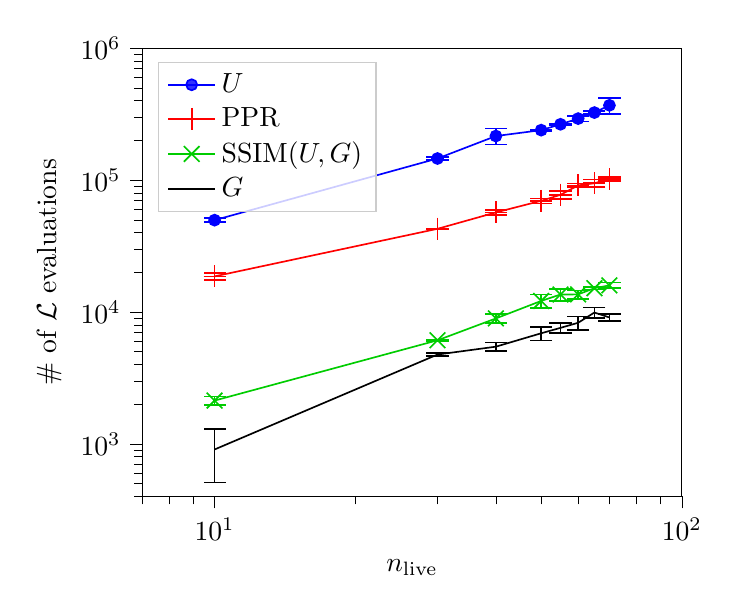
\begin{tikzpicture}

\definecolor{color0}{rgb}{0.0,0.0,1.0} %U
\definecolor{color1}{rgb}{1,0.0,0.0} %PPR
\definecolor{color2}{rgb}{0,0.8,0.0}                              %SSIM
\definecolor{color3}{rgb}{0.,0.0,0.0} %G

\begin{axis}[
legend cell align={left},
legend style={fill opacity=0.8, draw opacity=1, text opacity=1, at={(0.03,0.97)}, anchor=north west, draw=white!80!black},
tick align=outside,
tick pos=left,
x grid style={white!69.0196078431373!black},
xlabel={\(n_\text{live}\)},
xmin=7, xmax=100,
xtick style={color=black},
y grid style={white!69.0196078431373!black},
ylabel={\# of \({\cal L}\) evaluations},
ymin=400, ymax=1000000.0,
ytick style={color=black},
xmode=log,
ymode=log
]
\path [draw=color0, semithick]
(axis cs:10,48051.1762746562)
--(axis cs:10,51361.4903920105);

\path [draw=color0, semithick]
(axis cs:30,141787.579248368)
--(axis cs:30,149701.087418299);

\path [draw=color0, semithick]
(axis cs:40,185671.527674282)
--(axis cs:40,245784.472325718);

\path [draw=color0, semithick]
(axis cs:50,236296.832694899)
--(axis cs:50,241822.500638435);

\path [draw=color0, semithick]
(axis cs:55,262655.71356965)
--(axis cs:55,266952.953097016);

\path [draw=color0, semithick]
(axis cs:60,278243.015081106)
--(axis cs:60,306644.984918894);

\path [draw=color0, semithick]
(axis cs:65,317116.521541605)
--(axis cs:65,332736.145125062);

\path [draw=color0, semithick]
(axis cs:70,318358.948415036)
--(axis cs:70,419081.71825163);

\path [draw=color1, semithick]
(axis cs:10,17520.6487596482)
--(axis cs:10,19742.0179070185);

\path [draw=color1, semithick]
(axis cs:30,42472.9620658463)
--(axis cs:30,42994.371267487);

\path [draw=color1, semithick]
(axis cs:40,54281.6999405287)
--(axis cs:40,59494.3000594713);

\path [draw=color1, semithick]
(axis cs:50,66559.0160569084)
--(axis cs:50,72717.6506097582);

\path [draw=color1, semithick]
(axis cs:55,71552.6011973656)
--(axis cs:55,83118.7321359677);

\path [draw=color1, semithick]
(axis cs:60,88312.8386239607)
--(axis cs:60,94072.4947093726);

\path [draw=color1, semithick]
(axis cs:65,88215.9096228476)
--(axis cs:65,100992.090377152);

\path [draw=color1, semithick]
(axis cs:70,97882.04633)
--(axis cs:70,105637.95367);

\path [draw=color2, semithick]
(axis cs:10,1980.99743591911)
--(axis cs:10,2284.33589741422);

\path [draw=color2, semithick]
(axis cs:30,6035.87692136486)
--(axis cs:30,6174.12307863514);

\path [draw=color2, semithick]
(axis cs:40,8260.41435100755)
--(axis cs:40,9624.91898232578);

\path [draw=color2, semithick]
(axis cs:50,10733.0849396109)
--(axis cs:50,13538.9150603891);

\path [draw=color2, semithick]
(axis cs:55,12122.9645002052)
--(axis cs:55,15015.0354997948);

\path [draw=color2, semithick]
(axis cs:60,12622.7721075812)
--(axis cs:60,14593.2278924188);

\path [draw=color2, semithick]
(axis cs:65,14804.9685728395)
--(axis cs:65,15505.0314271605);

\path [draw=color2, semithick]
(axis cs:70,15158.1193669152)
--(axis cs:70,16693.8806330848);

\path [draw=color3, semithick]
(axis cs:10,511.628293172651)
--(axis cs:10,1305.03837349402);

\path [draw=color3, semithick]
(axis cs:30,4625.34584399058)
--(axis cs:30,4900.65415600942);

\path [draw=color3, semithick]
(axis cs:40,5045.39013421616)
--(axis cs:40,5880.60986578384);

\path [draw=color3, semithick]
(axis cs:50,6085.69651897324)
--(axis cs:50,7719.6368143601);

\path [draw=color3, semithick]
(axis cs:55,6959.0338647499)
--(axis cs:55,8215.63280191676);

\path [draw=color3, semithick]
(axis cs:60,7317.2571539732)
--(axis cs:60,9267.40951269347);

\path [draw=color3, semithick]
(axis cs:65,8986.02980736454)
--(axis cs:65,10838.6368593021);

\path [draw=color3, semithick]
(axis cs:70,8588.48027282128)
--(axis cs:70,9612.18639384539);


\addplot [semithick, color1, mark=-, mark size=4, mark options={solid}, only marks, forget plot]
table {%
10 17520.6487596482
30 42472.9620658463
40 54281.6999405287
50 66559.0160569084
55 71552.6011973656
60 88312.8386239607
65 88215.9096228476
70 97882.04633
};
\addplot [semithick, color1, mark=-, mark size=4, mark options={solid}, only marks, forget plot]
table {%
10 19742.0179070185
30 42994.371267487
40 59494.3000594713
50 72717.6506097582
55 83118.7321359677
60 94072.4947093726
65 100992.090377152
70 105637.95367
};
\addplot [semithick, color2, mark=-, mark size=4, mark options={solid}, only marks, forget plot]
table {%
10 1980.99743591911
30 6035.87692136486
40 8260.41435100755
50 10733.0849396109
55 12122.9645002052
60 12622.7721075812
65 14804.9685728395
70 15158.1193669152
};
\addplot [semithick, color2, mark=-, mark size=4, mark options={solid}, only marks, forget plot]
table {%
10 2284.33589741422
30 6174.12307863514
40 9624.91898232578
50 13538.9150603891
55 15015.0354997948
60 14593.2278924188
65 15505.0314271605
70 16693.8806330848
};
\addplot [semithick, color3, mark=-, mark size=4, mark options={solid}, only marks, forget plot]
table {%
10 511.628293172651
30 4625.34584399058
40 5045.39013421616
50 6085.69651897324
55 6959.0338647499
60 7317.2571539732
65 8986.02980736454
70 8588.48027282128
};
\addplot [semithick, color3, mark=-, mark size=4, mark options={solid}, only marks, forget plot]
table {%
10 1305.03837349402
30 4900.65415600942
40 5880.60986578384
50 7719.6368143601
55 8215.63280191676
60 9267.40951269347
65 10838.6368593021
70 9612.18639384539
};
\addplot [semithick, color0, mark=-, mark size=4, mark options={solid}, only marks, forget plot]
table {%
10 48051.1762746562
30 141787.579248368
40 185671.527674282
50 236296.832694899
55 262655.71356965
60 278243.015081106
65 317116.521541605
70 318358.948415036
};
\addplot [semithick, color0, mark=-, mark size=4, mark options={solid}, only marks, forget plot]
table {%
10 51361.4903920105
30 149701.087418299
40 245784.472325718
50 241822.500638435
55 266952.953097016
60 306644.984918894
65 332736.145125062
70 419081.71825163
};
\addplot [semithick, color0, mark=*, mark size=2, mark options={solid}]
table {%
10 49706.3333333333
30 145744.333333333
40 215728
50 239059.666666667
55 264804.333333333
60 292444
65 324926.333333333
70 368720.333333333
};
\addlegendentry{$U$}
\addplot [semithick, color1, mark=+, mark size=4, mark options={solid}]
table {%
10 18631.3333333333
30 42733.6666666667
40 56888
50 69638.3333333333
55 77335.6666666667
60 91192.6666666667
65 94604
70 101760
};
\addlegendentry{PPR}
\addplot [semithick, color2, mark=x, mark size=4, mark options={solid}]
table {%
10 2132.66666666667
30 6105
40 8942.66666666667
50 12136
55 13569
60 13608
65 15155
70 15926
};
\addlegendentry{$\text{SSIM}(U,G)$}
\addplot [semithick, color3, mark=., mark size=2, mark options={solid}]
table {%
10 908.333333333333
30 4763
40 5463
50 6902.66666666667
55 7587.33333333333
60 8292.33333333333
65 9912.33333333333
70 9100.33333333333
};
\addlegendentry{$G$}
\end{axis}

\end{tikzpicture}

\end{figure}
\end{frame}

\begin{frame}[label={sec:org34912c4}]{And Accurate.}
\begin{figure}
% This file was created by tikzplotlib v0.9.1.
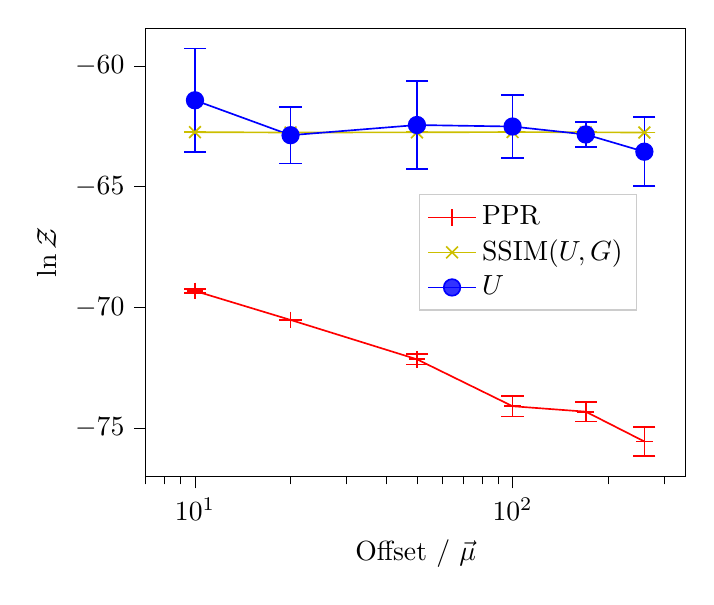
\begin{tikzpicture}

\definecolor{color0}{rgb}{1,0.0,0.0}
\definecolor{color1}{rgb}{0.8,0.75,0.0}
\definecolor{color2}{rgb}{0.0,0.0,1}

\begin{axis}[
legend cell align={left},
legend style={fill opacity=0.8, draw opacity=1, text opacity=1, at={(0.91,0.5)}, anchor=east, draw=white!80!black},
tick align=outside,
tick pos=left,
x grid style={white!69.0196078431373!black},
xlabel={Offset / \(\displaystyle \vec{\mu}\)},
xmin=-2.5, xmax=350.5,
xtick style={color=black},
y grid style={white!69.0196078431373!black},
ylabel={\(\displaystyle \ln {\cal Z}\)},
ymin=-77.013439988999, ymax=-58.4325947574349,
ytick style={color=black},
xmode=log
]
\path [draw=color0, semithick]
(axis cs:10,-69.4059960469118)
--(axis cs:10,-69.2379297037398);

\path [draw=color0, semithick]
(axis cs:20,-70.5299156173721)
--(axis cs:20,-70.5157474991409);

\path [draw=color0, semithick]
(axis cs:50,-72.3755951664078)
--(axis cs:50,-71.9328145858461);

\path [draw=color0, semithick]
(axis cs:100,-74.5305277482911)
--(axis cs:100,-73.6673769114354);

\path [draw=color0, semithick]
(axis cs:170,-74.7380053024013)
--(axis cs:170,-73.9121550603194);

\path [draw=color0, semithick]
(axis cs:260,-76.168856114837)
--(axis cs:260,-74.9518470928008);

\path [draw=color1, semithick]
(axis cs:10,-62.7439928102151)
--(axis cs:10,-62.7359696372663);

\path [draw=color1, semithick]
(axis cs:20,-62.755485458383)
--(axis cs:20,-62.7535773275597);

\path [draw=color1, semithick]
(axis cs:50,-62.7484141957878)
--(axis cs:50,-62.7468638775576);

\path [draw=color1, semithick]
(axis cs:100,-62.7369486572665)
--(axis cs:100,-62.7333125352419);

\path [draw=color1, semithick]
(axis cs:170,-62.746863877575)
--(axis cs:170,-62.745391448683);

\path [draw=color1, semithick]
(axis cs:260,-62.7574960930232)
--(axis cs:260,-62.7517661617973);

\path [draw=color2, semithick]
(axis cs:10,-63.5623386499016)
--(axis cs:10,-59.2771786315969);

\path [draw=color2, semithick]
(axis cs:20,-64.0348662974579)
--(axis cs:20,-61.6973543628668);

\path [draw=color2, semithick]
(axis cs:50,-64.2749108611421)
--(axis cs:50,-60.6135450768888);

\path [draw=color2, semithick]
(axis cs:100,-63.8144479355573)
--(axis cs:100,-61.1997313352197);

\path [draw=color2, semithick]
(axis cs:170,-63.3536082125541)
--(axis cs:170,-62.3180044247467);

\path [draw=color2, semithick]
(axis cs:260,-64.9781441262723)
--(axis cs:260,-62.1236339929356);

\addplot [semithick, color0, mark=-, mark size=4, mark options={solid}, only marks, forget plot]
table {%
10 -69.4059960469118
20 -70.5299156173721
50 -72.3755951664078
100 -74.5305277482911
170 -74.7380053024013
260 -76.168856114837
};
\addplot [semithick, color0, mark=-, mark size=4, mark options={solid}, only marks, forget plot]
table {%
10 -69.2379297037398
20 -70.5157474991409
50 -71.9328145858461
100 -73.6673769114354
170 -73.9121550603194
260 -74.9518470928008
};
\addplot [semithick, color1, mark=-, mark size=4, mark options={solid}, only marks, forget plot]
table {%
10 -62.7439928102151
20 -62.755485458383
50 -62.7484141957878
100 -62.7369486572665
170 -62.746863877575
260 -62.7574960930232
};
\addplot [semithick, color1, mark=-, mark size=4, mark options={solid}, only marks, forget plot]
table {%
10 -62.7359696372663
20 -62.7535773275597
50 -62.7468638775576
100 -62.7333125352419
170 -62.745391448683
260 -62.7517661617973
};
\addplot [semithick, color2, mark=-, mark size=4, mark options={solid}, only marks, forget plot]
table {%
10 -63.5623386499016
20 -64.0348662974579
50 -64.2749108611421
100 -63.8144479355573
170 -63.3536082125541
260 -64.9781441262723
};
\addplot [semithick, color2, mark=-, mark size=4, mark options={solid}, only marks, forget plot]
table {%
10 -59.2771786315969
20 -61.6973543628668
50 -60.6135450768888
100 -61.1997313352197
170 -62.3180044247467
260 -62.1236339929356
};
\addplot [semithick, color0, mark=+, mark size=3, mark options={solid}]
table {%
10 -69.3219628753258
20 -70.5228315582565
50 -72.154204876127
100 -74.0989523298633
170 -74.3250801813604
260 -75.5603516038189
};
\addlegendentry{PPR}
\addplot [semithick, color1, mark=x, mark size=3, mark options={solid}]
table {%
10 -62.7399812237407
20 -62.7545313929713
50 -62.7476390366727
100 -62.7351305962542
170 -62.746127663129
260 -62.7546311274102
};
\addlegendentry{SSIM$(U, G)$}
\addplot [semithick, color2, mark=*, mark size=3, mark options={solid}]
table {%
10 -61.4197586407493
20 -62.8661103301623
50 -62.4442279690155
100 -62.5070896353885
170 -62.8358063186504
260 -63.5508890596039
};
\addlegendentry{$U$}
\end{axis}

\end{tikzpicture}

\end{figure}
\end{frame}

\begin{frame}[fragile,label={sec:org7a68446}]{What this can do?}
 Examples: 
\begin{itemize}
\item Can accelerate if you know \alert{roughly} what to expect.
\item Can make more robust if you are wrong about the where.
\item Can make more robust if you are unsure about biases.
\item This can allow you to chain models.
\item You can run a \texttt{CosmoChord} on a laptop, \texttt{Cobaya} on a desktop.
\end{itemize}
\end{frame}
\end{document}